% Options for packages loaded elsewhere
\PassOptionsToPackage{unicode}{hyperref}
\PassOptionsToPackage{hyphens}{url}
%
\documentclass[
]{article}
\usepackage{lmodern}
\usepackage{amssymb,amsmath}
\usepackage{ifxetex,ifluatex}
\ifnum 0\ifxetex 1\fi\ifluatex 1\fi=0 % if pdftex
  \usepackage[T1]{fontenc}
  \usepackage[utf8]{inputenc}
  \usepackage{textcomp} % provide euro and other symbols
\else % if luatex or xetex
  \usepackage{unicode-math}
  \defaultfontfeatures{Scale=MatchLowercase}
  \defaultfontfeatures[\rmfamily]{Ligatures=TeX,Scale=1}
\fi
% Use upquote if available, for straight quotes in verbatim environments
\IfFileExists{upquote.sty}{\usepackage{upquote}}{}
\IfFileExists{microtype.sty}{% use microtype if available
  \usepackage[]{microtype}
  \UseMicrotypeSet[protrusion]{basicmath} % disable protrusion for tt fonts
}{}
\makeatletter
\@ifundefined{KOMAClassName}{% if non-KOMA class
  \IfFileExists{parskip.sty}{%
    \usepackage{parskip}
  }{% else
    \setlength{\parindent}{0pt}
    \setlength{\parskip}{6pt plus 2pt minus 1pt}}
}{% if KOMA class
  \KOMAoptions{parskip=half}}
\makeatother
\usepackage{xcolor}
\IfFileExists{xurl.sty}{\usepackage{xurl}}{} % add URL line breaks if available
\IfFileExists{bookmark.sty}{\usepackage{bookmark}}{\usepackage{hyperref}}
\hypersetup{
  pdftitle={RNA-Seq Data Analysis},
  pdfauthor={Wilbur Ouma},
  hidelinks,
  pdfcreator={LaTeX via pandoc}}
\urlstyle{same} % disable monospaced font for URLs
\usepackage[margin=1in]{geometry}
\usepackage{color}
\usepackage{fancyvrb}
\newcommand{\VerbBar}{|}
\newcommand{\VERB}{\Verb[commandchars=\\\{\}]}
\DefineVerbatimEnvironment{Highlighting}{Verbatim}{commandchars=\\\{\}}
% Add ',fontsize=\small' for more characters per line
\usepackage{framed}
\definecolor{shadecolor}{RGB}{248,248,248}
\newenvironment{Shaded}{\begin{snugshade}}{\end{snugshade}}
\newcommand{\AlertTok}[1]{\textcolor[rgb]{0.94,0.16,0.16}{#1}}
\newcommand{\AnnotationTok}[1]{\textcolor[rgb]{0.56,0.35,0.01}{\textbf{\textit{#1}}}}
\newcommand{\AttributeTok}[1]{\textcolor[rgb]{0.77,0.63,0.00}{#1}}
\newcommand{\BaseNTok}[1]{\textcolor[rgb]{0.00,0.00,0.81}{#1}}
\newcommand{\BuiltInTok}[1]{#1}
\newcommand{\CharTok}[1]{\textcolor[rgb]{0.31,0.60,0.02}{#1}}
\newcommand{\CommentTok}[1]{\textcolor[rgb]{0.56,0.35,0.01}{\textit{#1}}}
\newcommand{\CommentVarTok}[1]{\textcolor[rgb]{0.56,0.35,0.01}{\textbf{\textit{#1}}}}
\newcommand{\ConstantTok}[1]{\textcolor[rgb]{0.00,0.00,0.00}{#1}}
\newcommand{\ControlFlowTok}[1]{\textcolor[rgb]{0.13,0.29,0.53}{\textbf{#1}}}
\newcommand{\DataTypeTok}[1]{\textcolor[rgb]{0.13,0.29,0.53}{#1}}
\newcommand{\DecValTok}[1]{\textcolor[rgb]{0.00,0.00,0.81}{#1}}
\newcommand{\DocumentationTok}[1]{\textcolor[rgb]{0.56,0.35,0.01}{\textbf{\textit{#1}}}}
\newcommand{\ErrorTok}[1]{\textcolor[rgb]{0.64,0.00,0.00}{\textbf{#1}}}
\newcommand{\ExtensionTok}[1]{#1}
\newcommand{\FloatTok}[1]{\textcolor[rgb]{0.00,0.00,0.81}{#1}}
\newcommand{\FunctionTok}[1]{\textcolor[rgb]{0.00,0.00,0.00}{#1}}
\newcommand{\ImportTok}[1]{#1}
\newcommand{\InformationTok}[1]{\textcolor[rgb]{0.56,0.35,0.01}{\textbf{\textit{#1}}}}
\newcommand{\KeywordTok}[1]{\textcolor[rgb]{0.13,0.29,0.53}{\textbf{#1}}}
\newcommand{\NormalTok}[1]{#1}
\newcommand{\OperatorTok}[1]{\textcolor[rgb]{0.81,0.36,0.00}{\textbf{#1}}}
\newcommand{\OtherTok}[1]{\textcolor[rgb]{0.56,0.35,0.01}{#1}}
\newcommand{\PreprocessorTok}[1]{\textcolor[rgb]{0.56,0.35,0.01}{\textit{#1}}}
\newcommand{\RegionMarkerTok}[1]{#1}
\newcommand{\SpecialCharTok}[1]{\textcolor[rgb]{0.00,0.00,0.00}{#1}}
\newcommand{\SpecialStringTok}[1]{\textcolor[rgb]{0.31,0.60,0.02}{#1}}
\newcommand{\StringTok}[1]{\textcolor[rgb]{0.31,0.60,0.02}{#1}}
\newcommand{\VariableTok}[1]{\textcolor[rgb]{0.00,0.00,0.00}{#1}}
\newcommand{\VerbatimStringTok}[1]{\textcolor[rgb]{0.31,0.60,0.02}{#1}}
\newcommand{\WarningTok}[1]{\textcolor[rgb]{0.56,0.35,0.01}{\textbf{\textit{#1}}}}
\usepackage{graphicx,grffile}
\makeatletter
\def\maxwidth{\ifdim\Gin@nat@width>\linewidth\linewidth\else\Gin@nat@width\fi}
\def\maxheight{\ifdim\Gin@nat@height>\textheight\textheight\else\Gin@nat@height\fi}
\makeatother
% Scale images if necessary, so that they will not overflow the page
% margins by default, and it is still possible to overwrite the defaults
% using explicit options in \includegraphics[width, height, ...]{}
\setkeys{Gin}{width=\maxwidth,height=\maxheight,keepaspectratio}
% Set default figure placement to htbp
\makeatletter
\def\fps@figure{htbp}
\makeatother
\setlength{\emergencystretch}{3em} % prevent overfull lines
\providecommand{\tightlist}{%
  \setlength{\itemsep}{0pt}\setlength{\parskip}{0pt}}
\setcounter{secnumdepth}{-\maxdimen} % remove section numbering

\title{RNA-Seq Data Analysis}
\author{Wilbur Ouma}
\date{}

\begin{document}
\maketitle

\begin{center}\rule{0.5\linewidth}{0.5pt}\end{center}

\begin{quote}
\hypertarget{learning-objectives}{%
\subsubsection{Learning Objectives}\label{learning-objectives}}

\begin{itemize}
\item
  Define the following terms as they relate to R: object, assign, call,
  function, arguments, options.
\item
  Assign values to objects in R.
\item
  Learn how to \emph{name} objects
\item
  Use comments to inform script.
\item
  Solve simple arithmetic operations in R.
\item
  Call functions and use arguments to change their default options.
\item
  Inspect the content of vectors and manipulate their content.
\item
  Subset and extract values from vectors.
\item ~
  \hypertarget{analyze-vectors-with-missing-data.}{%
  \subsection{Analyze vectors with missing
  data.}\label{analyze-vectors-with-missing-data.}}
\end{itemize}
\end{quote}

\#\#NEW TO R? CHECK THESE OUT:
\url{https://datacarpentry.org/R-ecology-lesson/index.html} Data
wrangling cheatsheet:
\url{https://rstudio.com/wp-content/uploads/2015/02/data-wrangling-cheatsheet.pdf}
edgeR user guide:
\url{https://www.bioconductor.org/packages/release/bioc/vignettes/edgeR/inst/doc/edgeRUsersGuide.pdf}

RESEARCH QUESTION: What's the effect of salinity on gene expression?
What's of interest: the difference in treatement, rather than location

\#Adapted largely from:
\#\url{https://www.ncbi.nlm.nih.gov/pmc/articles/PMC4934518/pdf/f1000research-5-9996.pdf}

\#load(``RNASeq.RData'') \#install `Rsubread' package. DO ONCE! \#if
(!requireNamespace(``BiocManager'', quietly = TRUE)) \#
install.packages(``BiocManager'')

\#install.packages(``gplots'')

\#install `edgeR' \#BiocManager::install(``edgeR'')

\begin{Shaded}
\begin{Highlighting}[]
\KeywordTok{library}\NormalTok{(edgeR) }\CommentTok{#For DE analysis}
\end{Highlighting}
\end{Shaded}

\begin{verbatim}
## Loading required package: limma
\end{verbatim}

\#install data wrangling tools: \#install.packages(``tidyverse'')

\begin{Shaded}
\begin{Highlighting}[]
\KeywordTok{library}\NormalTok{(tidyverse) }\CommentTok{#includes ggplot2, dplyr, tidy, readr}
\end{Highlighting}
\end{Shaded}

\begin{verbatim}
## -- Attaching packages ------------------------------------------------------ tidyverse 1.3.0 --
\end{verbatim}

\begin{verbatim}
## v ggplot2 3.3.1     v purrr   0.3.4
## v tibble  3.0.1     v dplyr   1.0.0
## v tidyr   1.1.0     v stringr 1.4.0
## v readr   1.3.1     v forcats 0.5.0
\end{verbatim}

\begin{verbatim}
## -- Conflicts --------------------------------------------------------- tidyverse_conflicts() --
## x dplyr::filter() masks stats::filter()
## x dplyr::lag()    masks stats::lag()
\end{verbatim}

read in the raw counts

\begin{Shaded}
\begin{Highlighting}[]
\NormalTok{raw_counts <-}\StringTok{ }\KeywordTok{read.table}\NormalTok{(}\DataTypeTok{file=}\StringTok{"../gene_counts.txt"}\NormalTok{, }
                         \DataTypeTok{sep =} \StringTok{"}\CharTok{\textbackslash{}t}\StringTok{"}\NormalTok{, }
                         \DataTypeTok{header =} \OtherTok{TRUE}
\NormalTok{)}
\end{Highlighting}
\end{Shaded}

This is a data frame - first 6 columns contain information about the
features (genes),

\begin{Shaded}
\begin{Highlighting}[]
\KeywordTok{head}\NormalTok{(raw_counts)}
\end{Highlighting}
\end{Shaded}

\begin{verbatim}
##                  Geneid   Chr  Start    End Strand Length SRR7609467 SRR7609468
## 1 Phvul.001G000100.v1.0 Chr01   3852  11015      -   7164        138        123
## 2 Phvul.001G000200.v1.0 Chr01  99177 104451      -   5275          0          0
## 3 Phvul.001G000300.v1.0 Chr01 125452 132387      +   6936       3458       3530
## 4 Phvul.001G000400.v1.0 Chr01 134609 140566      -   5958        237        258
## 5 Phvul.001G000500.v1.0 Chr01 144309 146169      +   1861       1624       1351
## 6 Phvul.001G000600.v1.0 Chr01 149887 162657      +  12771        329        351
##   SRR7609469 SRR7609470 SRR7609471 SRR7609472 SRR7609473 SRR7609474 SRR7609475
## 1        142        154        116        128        133        132        111
## 2          0          0          0          0          0          0          0
## 3       3742       3979       3339       2912       3597       4190       3329
## 4        236        259        207        216        309        252        214
## 5       1650       1955       1551        902       1639       2136       1908
## 6        363        384        404        230        406        370        411
##   SRR7609476 SRR7609477 SRR7609478
## 1         91        116        147
## 2          0          0          0
## 3       3433       2652       3121
## 4        208        172        221
## 5       1701        621        730
## 6        359        185        232
\end{verbatim}

\#\#GO OVER STUDY DESIGN: WHAT QUESTIONS CAN BE ANSWERED BY THIS DESIGN?

add more informative row names IT: inland treated; IC: inland control;
BT: beach treated; BC: beach control

\begin{Shaded}
\begin{Highlighting}[]
\KeywordTok{names}\NormalTok{(raw_counts)[}\DecValTok{7}\OperatorTok{:}\DecValTok{18}\NormalTok{] <-}\StringTok{ }\KeywordTok{c}\NormalTok{(}\StringTok{"IT2"}\NormalTok{, }\StringTok{"BC2"}\NormalTok{, }\StringTok{"IC3"}\NormalTok{, }\StringTok{"IT1"}\NormalTok{, }\StringTok{"BC3"}\NormalTok{, }\StringTok{"BT1"}\NormalTok{, }\StringTok{"BC1"}\NormalTok{, }\StringTok{"IT3"}\NormalTok{, }\StringTok{"IC1"}\NormalTok{, }\StringTok{"IC2"}\NormalTok{, }\StringTok{"BT2"}\NormalTok{, }\StringTok{"BT3"}\NormalTok{)}

\KeywordTok{head}\NormalTok{(raw_counts)}
\end{Highlighting}
\end{Shaded}

\begin{verbatim}
##                  Geneid   Chr  Start    End Strand Length  IT2  BC2  IC3  IT1
## 1 Phvul.001G000100.v1.0 Chr01   3852  11015      -   7164  138  123  142  154
## 2 Phvul.001G000200.v1.0 Chr01  99177 104451      -   5275    0    0    0    0
## 3 Phvul.001G000300.v1.0 Chr01 125452 132387      +   6936 3458 3530 3742 3979
## 4 Phvul.001G000400.v1.0 Chr01 134609 140566      -   5958  237  258  236  259
## 5 Phvul.001G000500.v1.0 Chr01 144309 146169      +   1861 1624 1351 1650 1955
## 6 Phvul.001G000600.v1.0 Chr01 149887 162657      +  12771  329  351  363  384
##    BC3  BT1  BC1  IT3  IC1  IC2  BT2  BT3
## 1  116  128  133  132  111   91  116  147
## 2    0    0    0    0    0    0    0    0
## 3 3339 2912 3597 4190 3329 3433 2652 3121
## 4  207  216  309  252  214  208  172  221
## 5 1551  902 1639 2136 1908 1701  621  730
## 6  404  230  406  370  411  359  185  232
\end{verbatim}

reorder the columns to group treatments together, for each lo

\begin{Shaded}
\begin{Highlighting}[]
\NormalTok{raw_counts <-}\StringTok{ }\NormalTok{raw_counts[ , }\KeywordTok{c}\NormalTok{(}\DecValTok{1}\OperatorTok{:}\DecValTok{6}\NormalTok{, }\DecValTok{9}\NormalTok{,}\DecValTok{15}\NormalTok{,}\DecValTok{16}\NormalTok{,}\DecValTok{7}\NormalTok{,}\DecValTok{10}\NormalTok{,}\DecValTok{14}\NormalTok{,}\DecValTok{8}\NormalTok{,}\DecValTok{11}\NormalTok{,}\DecValTok{13}\NormalTok{,}\DecValTok{12}\NormalTok{,}\DecValTok{17}\NormalTok{,}\DecValTok{18}\NormalTok{)]}
\KeywordTok{head}\NormalTok{(raw_counts)}
\end{Highlighting}
\end{Shaded}

\begin{verbatim}
##                  Geneid   Chr  Start    End Strand Length  IC3  IC1  IC2  IT2
## 1 Phvul.001G000100.v1.0 Chr01   3852  11015      -   7164  142  111   91  138
## 2 Phvul.001G000200.v1.0 Chr01  99177 104451      -   5275    0    0    0    0
## 3 Phvul.001G000300.v1.0 Chr01 125452 132387      +   6936 3742 3329 3433 3458
## 4 Phvul.001G000400.v1.0 Chr01 134609 140566      -   5958  236  214  208  237
## 5 Phvul.001G000500.v1.0 Chr01 144309 146169      +   1861 1650 1908 1701 1624
## 6 Phvul.001G000600.v1.0 Chr01 149887 162657      +  12771  363  411  359  329
##    IT1  IT3  BC2  BC3  BC1  BT1  BT2  BT3
## 1  154  132  123  116  133  128  116  147
## 2    0    0    0    0    0    0    0    0
## 3 3979 4190 3530 3339 3597 2912 2652 3121
## 4  259  252  258  207  309  216  172  221
## 5 1955 2136 1351 1551 1639  902  621  730
## 6  384  370  351  404  406  230  185  232
\end{verbatim}

create the DGE object for edgeR

\begin{Shaded}
\begin{Highlighting}[]
\NormalTok{dge <-}\StringTok{ }\KeywordTok{DGEList}\NormalTok{(}\DataTypeTok{counts =}\NormalTok{ raw_counts[ , }\DecValTok{7}\OperatorTok{:}\DecValTok{18}\NormalTok{],}
               \DataTypeTok{lib.size =} \KeywordTok{colSums}\NormalTok{(raw_counts[ , }\DecValTok{7}\OperatorTok{:}\DecValTok{18}\NormalTok{]),}
               \DataTypeTok{norm.factors =} \KeywordTok{rep}\NormalTok{(}\DecValTok{1}\NormalTok{,}\KeywordTok{ncol}\NormalTok{(raw_counts[ , }\DecValTok{7}\OperatorTok{:}\DecValTok{18}\NormalTok{])),}
               \DataTypeTok{samples =} \OtherTok{NULL}\NormalTok{,}
               \DataTypeTok{group =} \OtherTok{NULL}\NormalTok{,}
               \DataTypeTok{genes =}\NormalTok{ raw_counts[ , }\DecValTok{1}\OperatorTok{:}\DecValTok{6}\NormalTok{])}


\NormalTok{dge}
\end{Highlighting}
\end{Shaded}

\begin{verbatim}
## An object of class "DGEList"
## $counts
##    IC3  IC1  IC2  IT2  IT1  IT3  BC2  BC3  BC1  BT1  BT2  BT3
## 1  142  111   91  138  154  132  123  116  133  128  116  147
## 2    0    0    0    0    0    0    0    0    0    0    0    0
## 3 3742 3329 3433 3458 3979 4190 3530 3339 3597 2912 2652 3121
## 4  236  214  208  237  259  252  258  207  309  216  172  221
## 5 1650 1908 1701 1624 1955 2136 1351 1551 1639  902  621  730
## 27192 more rows ...
## 
## $samples
##     group lib.size norm.factors
## IC3     1 40619905            1
## IC1     1 35114368            1
## IC2     1 34833786            1
## IT2     1 36399307            1
## IT1     1 41939123            1
## 7 more rows ...
## 
## $genes
##                  Geneid   Chr  Start    End Strand Length
## 1 Phvul.001G000100.v1.0 Chr01   3852  11015      -   7164
## 2 Phvul.001G000200.v1.0 Chr01  99177 104451      -   5275
## 3 Phvul.001G000300.v1.0 Chr01 125452 132387      +   6936
## 4 Phvul.001G000400.v1.0 Chr01 134609 140566      -   5958
## 5 Phvul.001G000500.v1.0 Chr01 144309 146169      +   1861
## 27192 more rows ...
\end{verbatim}

\begin{Shaded}
\begin{Highlighting}[]
\NormalTok{dge}\OperatorTok{$}\NormalTok{genes }\OperatorTok
\StringTok{  }\KeywordTok{head}\NormalTok{()}
\end{Highlighting}
\end{Shaded}

\begin{verbatim}
##                  Geneid   Chr  Start    End Strand Length
## 1 Phvul.001G000100.v1.0 Chr01   3852  11015      -   7164
## 2 Phvul.001G000200.v1.0 Chr01  99177 104451      -   5275
## 3 Phvul.001G000300.v1.0 Chr01 125452 132387      +   6936
## 4 Phvul.001G000400.v1.0 Chr01 134609 140566      -   5958
## 5 Phvul.001G000500.v1.0 Chr01 144309 146169      +   1861
## 6 Phvul.001G000600.v1.0 Chr01 149887 162657      +  12771
\end{verbatim}

\begin{Shaded}
\begin{Highlighting}[]
\NormalTok{dge}\OperatorTok{$}\NormalTok{samples}
\end{Highlighting}
\end{Shaded}

\begin{verbatim}
##     group lib.size norm.factors
## IC3     1 40619905            1
## IC1     1 35114368            1
## IC2     1 34833786            1
## IT2     1 36399307            1
## IT1     1 41939123            1
## IT3     1 42597147            1
## BC2     1 32496003            1
## BC3     1 31262960            1
## BC1     1 33240392            1
## BT1     1 31682364            1
## BT2     1 30170320            1
## BT3     1 34386767            1
\end{verbatim}

Add sample information:

\begin{Shaded}
\begin{Highlighting}[]
\NormalTok{treatment<-}\KeywordTok{as.factor}\NormalTok{(}\KeywordTok{rep}\NormalTok{(}\KeywordTok{c}\NormalTok{(}\StringTok{"IC"}\NormalTok{,}\StringTok{"IT"}\NormalTok{,}\StringTok{"BC"}\NormalTok{,}\StringTok{"BT"}\NormalTok{), }\KeywordTok{c}\NormalTok{(}\DecValTok{3}\NormalTok{,}\DecValTok{3}\NormalTok{,}\DecValTok{3}\NormalTok{,}\DecValTok{3}\NormalTok{)))}
\NormalTok{treatment }
\end{Highlighting}
\end{Shaded}

\begin{verbatim}
##  [1] IC IC IC IT IT IT BC BC BC BT BT BT
## Levels: BC BT IC IT
\end{verbatim}

Location

\begin{Shaded}
\begin{Highlighting}[]
\NormalTok{location<-}\KeywordTok{as.factor}\NormalTok{(}\KeywordTok{rep}\NormalTok{(}\KeywordTok{c}\NormalTok{(}\StringTok{"inland"}\NormalTok{,}\StringTok{"beach"}\NormalTok{),}\KeywordTok{c}\NormalTok{(}\DecValTok{6}\NormalTok{,}\DecValTok{6}\NormalTok{)))}
\NormalTok{location}
\end{Highlighting}
\end{Shaded}

\begin{verbatim}
##  [1] inland inland inland inland inland inland beach  beach  beach  beach 
## [11] beach  beach 
## Levels: beach inland
\end{verbatim}

\begin{Shaded}
\begin{Highlighting}[]
\NormalTok{dge}\OperatorTok{$}\NormalTok{samples}\OperatorTok{$}\NormalTok{group<-treatment}
\NormalTok{dge}\OperatorTok{$}\NormalTok{samples}\OperatorTok{$}\NormalTok{location<-location}
\NormalTok{dge}\OperatorTok{$}\NormalTok{samples}
\end{Highlighting}
\end{Shaded}

\begin{verbatim}
##     group lib.size norm.factors location
## IC3    IC 40619905            1   inland
## IC1    IC 35114368            1   inland
## IC2    IC 34833786            1   inland
## IT2    IT 36399307            1   inland
## IT1    IT 41939123            1   inland
## IT3    IT 42597147            1   inland
## BC2    BC 32496003            1    beach
## BC3    BC 31262960            1    beach
## BC1    BC 33240392            1    beach
## BT1    BT 31682364            1    beach
## BT2    BT 30170320            1    beach
## BT3    BT 34386767            1    beach
\end{verbatim}

make a copy:

\begin{Shaded}
\begin{Highlighting}[]
\NormalTok{dge_orig<-dge}
\end{Highlighting}
\end{Shaded}

\#\#\#\#\#DATA PRE-PROCESSING: \#\#AVOID RPKM!!! \#\#Transformations
from the raw-scale \#\#NOTE: \#\#CPM ``normalizaton'':

\begin{Shaded}
\begin{Highlighting}[]
\NormalTok{cpm <-}\StringTok{ }\KeywordTok{cpm}\NormalTok{(dge) }\CommentTok{##raw counts are converted to CPM and log-CPM values using the cpm function}
\NormalTok{lcpm <-}\StringTok{ }\KeywordTok{cpm}\NormalTok{(dge, }\DataTypeTok{log=}\OtherTok{TRUE}\NormalTok{)}

\NormalTok{L <-}\StringTok{ }\KeywordTok{mean}\NormalTok{(dge}\OperatorTok{$}\NormalTok{samples}\OperatorTok{$}\NormalTok{lib.size) }\OperatorTok{*}\StringTok{ }\FloatTok{1e-6} \CommentTok{#average library size in Millions}
\NormalTok{M <-}\StringTok{ }\KeywordTok{median}\NormalTok{(dge}\OperatorTok{$}\NormalTok{samples}\OperatorTok{$}\NormalTok{lib.size) }\OperatorTok{*}\StringTok{ }\FloatTok{1e-6} \CommentTok{#median lib size }

\KeywordTok{summary}\NormalTok{(lcpm)}
\end{Highlighting}
\end{Shaded}

\begin{verbatim}
##       IC3               IC1               IC2               IT2         
##  Min.   :-4.1455   Min.   :-4.1455   Min.   :-4.1455   Min.   :-4.1455  
##  1st Qu.:-0.8022   1st Qu.:-0.8132   1st Qu.:-0.8028   1st Qu.:-0.7227  
##  Median : 3.2078   Median : 3.2583   Median : 3.2173   Median : 3.3458  
##  Mean   : 2.2150   Mean   : 2.2433   Mean   : 2.2098   Mean   : 2.2857  
##  3rd Qu.: 5.1679   3rd Qu.: 5.2014   3rd Qu.: 5.1560   3rd Qu.: 5.2352  
##  Max.   :13.8265   Max.   :14.0279   Max.   :13.8234   Max.   :12.9911  
##       IT1               IT3               BC2               BC3         
##  Min.   :-4.1455   Min.   :-4.1455   Min.   :-4.1455   Min.   :-4.1455  
##  1st Qu.:-0.6694   1st Qu.:-0.7455   1st Qu.:-0.7868   1st Qu.:-0.8153  
##  Median : 3.3390   Median : 3.3302   Median : 3.2763   Median : 3.2946  
##  Mean   : 2.2830   Mean   : 2.2843   Mean   : 2.2288   Mean   : 2.2291  
##  3rd Qu.: 5.2276   3rd Qu.: 5.2360   3rd Qu.: 5.2016   3rd Qu.: 5.1945  
##  Max.   :13.2226   Max.   :13.1991   Max.   :13.8423   Max.   :13.9037  
##       BC1               BT1               BT2               BT3        
##  Min.   :-4.1455   Min.   :-4.1455   Min.   :-4.1455   Min.   :-4.145  
##  1st Qu.:-0.8162   1st Qu.:-0.9161   1st Qu.:-0.9419   1st Qu.:-0.786  
##  Median : 3.3153   Median : 3.2661   Median : 3.1971   Median : 3.284  
##  Mean   : 2.2502   Mean   : 2.2197   Mean   : 2.1812   Mean   : 2.241  
##  3rd Qu.: 5.2269   3rd Qu.: 5.2138   3rd Qu.: 5.1957   3rd Qu.: 5.211  
##  Max.   :12.6238   Max.   :12.9543   Max.   :12.7706   Max.   :13.004
\end{verbatim}

\begin{Shaded}
\begin{Highlighting}[]
\KeywordTok{summary}\NormalTok{(cpm)[,}\DecValTok{1}\OperatorTok{:}\DecValTok{3}\NormalTok{]}
\end{Highlighting}
\end{Shaded}

\begin{verbatim}
##       IC3                 IC1                 IC2           
##  Min.   :    0.000   Min.   :    0.000   Min.   :    0.000  
##  1st Qu.:    0.517   1st Qu.:    0.513   1st Qu.:    0.517  
##  Median :    9.183   Median :    9.512   Median :    9.244  
##  Mean   :   36.769   Mean   :   36.769   Mean   :   36.769  
##  3rd Qu.:   35.894   3rd Qu.:   36.737   3rd Qu.:   35.598  
##  Max.   :14527.705   Max.   :16703.447   Max.   :14496.414
\end{verbatim}

Removing genes that are lowly expressed get \# of genes with zero counts
across all samples:

\begin{Shaded}
\begin{Highlighting}[]
\KeywordTok{table}\NormalTok{(}\KeywordTok{rowSums}\NormalTok{(dge}\OperatorTok{$}\NormalTok{counts}\OperatorTok{==}\DecValTok{0}\NormalTok{)}\OperatorTok{==}\KeywordTok{ncol}\NormalTok{(dge}\OperatorTok{$}\NormalTok{counts)) }\CommentTok{#~10% of genes had count zero across all samples}
\end{Highlighting}
\end{Shaded}

\begin{verbatim}
## 
## FALSE  TRUE 
## 24655  2542
\end{verbatim}

Use the ``filterByExpr'' edgeR function. By default, the fxn keeps genes
with about 10 read counts or more in a minimum number of samples, where
the number of samples is chosen according to the minimum group sample
size. The actual filtering uses CPM values rather than counts in order
to avoid giving preference to samples with large library sizes. For
example, if the median library size is about 51 million and 10/51 ≈ 0.2,
so the filterByExpr function keeps genes that have a CPM of 0.2 or more
in at least three samples.

\begin{Shaded}
\begin{Highlighting}[]
\NormalTok{keep.exprs <-}\StringTok{ }\KeywordTok{filterByExpr}\NormalTok{(dge)}
\CommentTok{#NOTE: Consider adjusting the read count cutoff. By default, the function keeps genes with about 10 read counts or more in a minimum number of samples }
\CommentTok{#keep.exprs <- filterByExpr(dge, min.count = 5, min.total.count = 5)}

\NormalTok{dge <-}\StringTok{ }\NormalTok{dge[keep.exprs,, keep.lib.sizes=}\OtherTok{FALSE}\NormalTok{]}
\KeywordTok{dim}\NormalTok{(dge)}
\end{Highlighting}
\end{Shaded}

\begin{verbatim}
## [1] 21665    12
\end{verbatim}

\#\#LEARNING CHECK: WHAT proportion of TOTAL GENES ARE KEPT? Hide this
answer!

\begin{Shaded}
\begin{Highlighting}[]
\KeywordTok{dim}\NormalTok{(dge}\OperatorTok{$}\NormalTok{counts)[}\DecValTok{1}\NormalTok{]}\OperatorTok{/}\KeywordTok{dim}\NormalTok{(dge_orig}\OperatorTok{$}\NormalTok{counts)[}\DecValTok{1}\NormalTok{]}
\end{Highlighting}
\end{Shaded}

\begin{verbatim}
## [1] 0.7965952
\end{verbatim}

\#make plots

\begin{Shaded}
\begin{Highlighting}[]
\NormalTok{samplenames<-}\KeywordTok{c}\NormalTok{(}\StringTok{"Inland_c3"}\NormalTok{,}\StringTok{"Inland_c1"}\NormalTok{,}\StringTok{"Inland_c2"}\NormalTok{,}\StringTok{"Inland_t2"}\NormalTok{,}\StringTok{"Inland_t1"}\NormalTok{,}\StringTok{"Inland_t3"}\NormalTok{,}
               \StringTok{"Beach_c2"}\NormalTok{,}\StringTok{"Beach_c3"}\NormalTok{,}\StringTok{"Beach_c1"}\NormalTok{,}\StringTok{"Beach_t1"}\NormalTok{,}\StringTok{"Beach_t2"}\NormalTok{,}\StringTok{"Beach_t3"}\NormalTok{)}
\CommentTok{#Lib sizes:}
\KeywordTok{barplot}\NormalTok{(dge}\OperatorTok{$}\NormalTok{samples}\OperatorTok{$}\NormalTok{lib.size, }\DataTypeTok{las =} \DecValTok{2}\NormalTok{, }\DataTypeTok{names.arg =}\NormalTok{ samplenames)}
\end{Highlighting}
\end{Shaded}

\includegraphics{rna_seq_analysis_files/figure-latex/unnamed-chunk-15-1.pdf}

\begin{Shaded}
\begin{Highlighting}[]
\KeywordTok{library}\NormalTok{(RColorBrewer)}
\NormalTok{lcpm.cutoff <-}\StringTok{ }\KeywordTok{log2}\NormalTok{(}\DecValTok{10}\OperatorTok{/}\NormalTok{M }\OperatorTok{+}\StringTok{ }\DecValTok{2}\OperatorTok{/}\NormalTok{L)}
\NormalTok{nsamples <-}\StringTok{ }\KeywordTok{ncol}\NormalTok{(dge)}
\NormalTok{col <-}\StringTok{ }\KeywordTok{brewer.pal}\NormalTok{(nsamples, }\StringTok{"Paired"}\NormalTok{)}
\KeywordTok{par}\NormalTok{(}\DataTypeTok{mfrow=}\KeywordTok{c}\NormalTok{(}\DecValTok{1}\NormalTok{,}\DecValTok{2}\NormalTok{))}
\KeywordTok{plot}\NormalTok{(}\KeywordTok{density}\NormalTok{(lcpm[,}\DecValTok{1}\NormalTok{]), }\DataTypeTok{col=}\NormalTok{col[}\DecValTok{1}\NormalTok{], }\DataTypeTok{lwd=}\DecValTok{2}\NormalTok{, }\DataTypeTok{ylim=}\KeywordTok{c}\NormalTok{(}\DecValTok{0}\NormalTok{,}\FloatTok{0.26}\NormalTok{), }\DataTypeTok{las=}\DecValTok{2}\NormalTok{, }\DataTypeTok{main=}\StringTok{""}\NormalTok{, }\DataTypeTok{xlab=}\StringTok{""}\NormalTok{) }\CommentTok{#density with lcpm from unfiltered data}
\KeywordTok{title}\NormalTok{(}\DataTypeTok{main=}\StringTok{"A. Raw data"}\NormalTok{, }\DataTypeTok{xlab=}\StringTok{"Log-cpm"}\NormalTok{)}
\KeywordTok{abline}\NormalTok{(}\DataTypeTok{v=}\NormalTok{lcpm.cutoff, }\DataTypeTok{lty=}\DecValTok{3}\NormalTok{)}
\ControlFlowTok{for}\NormalTok{ (i }\ControlFlowTok{in} \DecValTok{2}\OperatorTok{:}\NormalTok{nsamples)\{}
\NormalTok{  den <-}\StringTok{ }\KeywordTok{density}\NormalTok{(lcpm[,i])}
  \KeywordTok{lines}\NormalTok{(den}\OperatorTok{$}\NormalTok{x, den}\OperatorTok{$}\NormalTok{y, }\DataTypeTok{col=}\NormalTok{col[i], }\DataTypeTok{lwd=}\DecValTok{2}\NormalTok{)}
\NormalTok{\}}
\CommentTok{#legend("topright", samplenames, text.col=col, bty="n")}
\NormalTok{lcpm2 <-}\StringTok{ }\KeywordTok{cpm}\NormalTok{(dge, }\DataTypeTok{log=}\OtherTok{TRUE}\NormalTok{) }\CommentTok{#NOTE: reculculating lcpm from filtered data!!! }
\KeywordTok{plot}\NormalTok{(}\KeywordTok{density}\NormalTok{(lcpm2[,}\DecValTok{1}\NormalTok{]), }\DataTypeTok{col=}\NormalTok{col[}\DecValTok{1}\NormalTok{], }\DataTypeTok{lwd=}\DecValTok{2}\NormalTok{, }\DataTypeTok{ylim=}\KeywordTok{c}\NormalTok{(}\DecValTok{0}\NormalTok{,}\FloatTok{0.26}\NormalTok{), }\DataTypeTok{las=}\DecValTok{2}\NormalTok{, }\DataTypeTok{main=}\StringTok{""}\NormalTok{, }\DataTypeTok{xlab=}\StringTok{""}\NormalTok{)}
\KeywordTok{title}\NormalTok{(}\DataTypeTok{main=}\StringTok{"B. Filtered data"}\NormalTok{, }\DataTypeTok{xlab=}\StringTok{"Log-cpm"}\NormalTok{)}
\KeywordTok{abline}\NormalTok{(}\DataTypeTok{v=}\NormalTok{lcpm.cutoff, }\DataTypeTok{lty=}\DecValTok{3}\NormalTok{)}
\ControlFlowTok{for}\NormalTok{ (i }\ControlFlowTok{in} \DecValTok{2}\OperatorTok{:}\NormalTok{nsamples)\{}
\NormalTok{  den <-}\StringTok{ }\KeywordTok{density}\NormalTok{(lcpm2[,i])}
  \KeywordTok{lines}\NormalTok{(den}\OperatorTok{$}\NormalTok{x, den}\OperatorTok{$}\NormalTok{y, }\DataTypeTok{col=}\NormalTok{col[i], }\DataTypeTok{lwd=}\DecValTok{2}\NormalTok{)}
\NormalTok{\}}
\end{Highlighting}
\end{Shaded}

\includegraphics{rna_seq_analysis_files/figure-latex/unnamed-chunk-15-2.pdf}

\begin{Shaded}
\begin{Highlighting}[]
\CommentTok{#legend("topright", samplenames, text.col=col, bty="n")}
\CommentTok{#dev.off()}
\end{Highlighting}
\end{Shaded}

\#Normalization for sequencing depth differences Normalization:

\begin{Shaded}
\begin{Highlighting}[]
\NormalTok{dge_unNorm<-dge }\CommentTok{#create a copy of unnormalized data}
\NormalTok{dge <-}\StringTok{ }\KeywordTok{calcNormFactors}\NormalTok{(dge, }\DataTypeTok{method =} \StringTok{"TMM"}\NormalTok{)}
\end{Highlighting}
\end{Shaded}

Changes in normalization factors:

\begin{Shaded}
\begin{Highlighting}[]
\NormalTok{dge}\OperatorTok{$}\NormalTok{samples}
\end{Highlighting}
\end{Shaded}

\begin{verbatim}
##     group lib.size norm.factors location
## IC3    IC 40613336    0.9618646   inland
## IC1    IC 35108304    0.9961767   inland
## IC2    IC 34828021    0.9549586   inland
## IT2    IT 36393071    1.0309439   inland
## IT1    IT 41932500    1.0306391   inland
## IT3    IT 42590205    1.0361333   inland
## BC2    BC 32491348    1.0085894    beach
## BC3    BC 31258594    1.0090062    beach
## BC1    BC 33235105    1.0393256    beach
## BT1    BT 31677628    0.9892230    beach
## BT2    BT 30165626    0.9587813    beach
## BT3    BT 34381220    0.9895421    beach
\end{verbatim}

Plot distribution of expression values, per sample:

\begin{Shaded}
\begin{Highlighting}[]
\KeywordTok{par}\NormalTok{(}\DataTypeTok{mfrow=}\KeywordTok{c}\NormalTok{(}\DecValTok{1}\NormalTok{,}\DecValTok{2}\NormalTok{))}

\NormalTok{lcpm <-}\StringTok{ }\KeywordTok{cpm}\NormalTok{(dge_unNorm, }\DataTypeTok{log=}\OtherTok{TRUE}\NormalTok{)}
\KeywordTok{boxplot}\NormalTok{(lcpm, }\DataTypeTok{las=}\DecValTok{2}\NormalTok{, }\DataTypeTok{col=}\NormalTok{col, }\DataTypeTok{main=}\StringTok{""}\NormalTok{)}
\KeywordTok{title}\NormalTok{(}\DataTypeTok{main=}\StringTok{"Unnormalized data"}\NormalTok{,}\DataTypeTok{ylab=}\StringTok{"Log-cpm"}\NormalTok{)}

\NormalTok{lcpm <-}\StringTok{ }\KeywordTok{cpm}\NormalTok{(dge, }\DataTypeTok{log=}\OtherTok{TRUE}\NormalTok{)}
\KeywordTok{boxplot}\NormalTok{(lcpm, }\DataTypeTok{las=}\DecValTok{2}\NormalTok{, }\DataTypeTok{col=}\NormalTok{col, }\DataTypeTok{main=}\StringTok{""}\NormalTok{)}
\KeywordTok{title}\NormalTok{(}\DataTypeTok{main=}\StringTok{"Normalized data"}\NormalTok{,}\DataTypeTok{ylab=}\StringTok{"Log-cpm"}\NormalTok{)}
\end{Highlighting}
\end{Shaded}

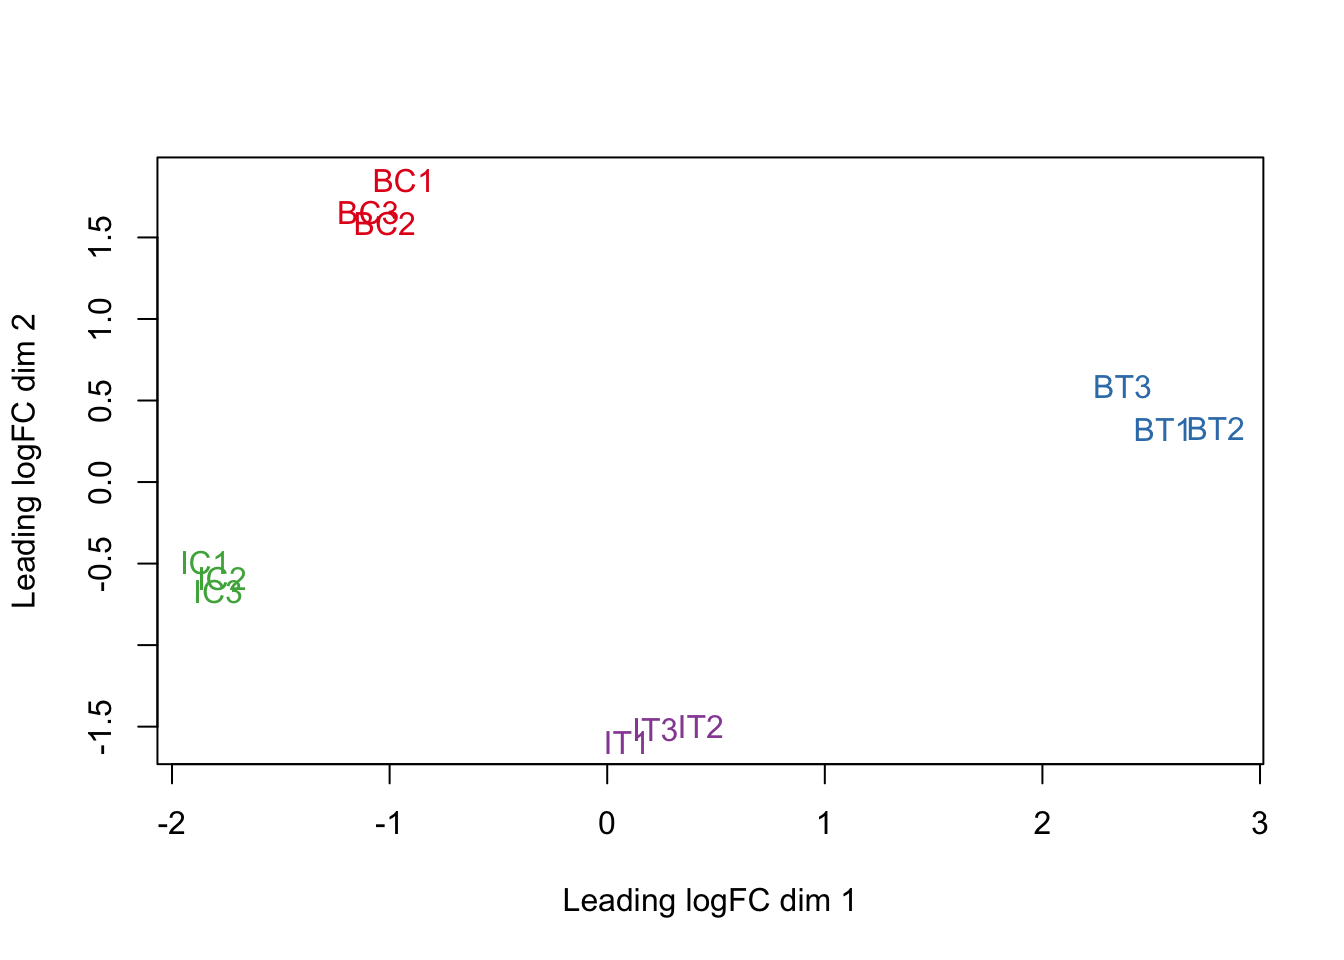
\includegraphics{rna_seq_analysis_files/figure-latex/unnamed-chunk-18-1.pdf}

\#MDS plots To create the MDS plots, we assign different colours to the
factors of interest. Dimensions 1 and 2 are examined using the colour
grouping (i.e treatment).

\begin{Shaded}
\begin{Highlighting}[]
\NormalTok{lcpm <-}\StringTok{ }\KeywordTok{cpm}\NormalTok{(dge, }\DataTypeTok{log=}\OtherTok{TRUE}\NormalTok{)}
\CommentTok{#par(mfrow=c(1,2))}
\NormalTok{col.group <-}\StringTok{ }\NormalTok{dge}\OperatorTok{$}\NormalTok{samples}\OperatorTok{$}\NormalTok{group}
\KeywordTok{levels}\NormalTok{(col.group) <-}\StringTok{ }\KeywordTok{brewer.pal}\NormalTok{(}\KeywordTok{nlevels}\NormalTok{(col.group), }\StringTok{"Set1"}\NormalTok{)}
\NormalTok{col.group <-}\StringTok{ }\KeywordTok{as.character}\NormalTok{(col.group)}
\CommentTok{#col.lane <- lane}
\CommentTok{#levels(col.lane) <- brewer.pal(nlevels(col.lane), "Set2")}
\CommentTok{#col.lane <- as.character(col.lane)}
\KeywordTok{plotMDS}\NormalTok{(lcpm, }\DataTypeTok{col=}\NormalTok{col.group) }
\end{Highlighting}
\end{Shaded}

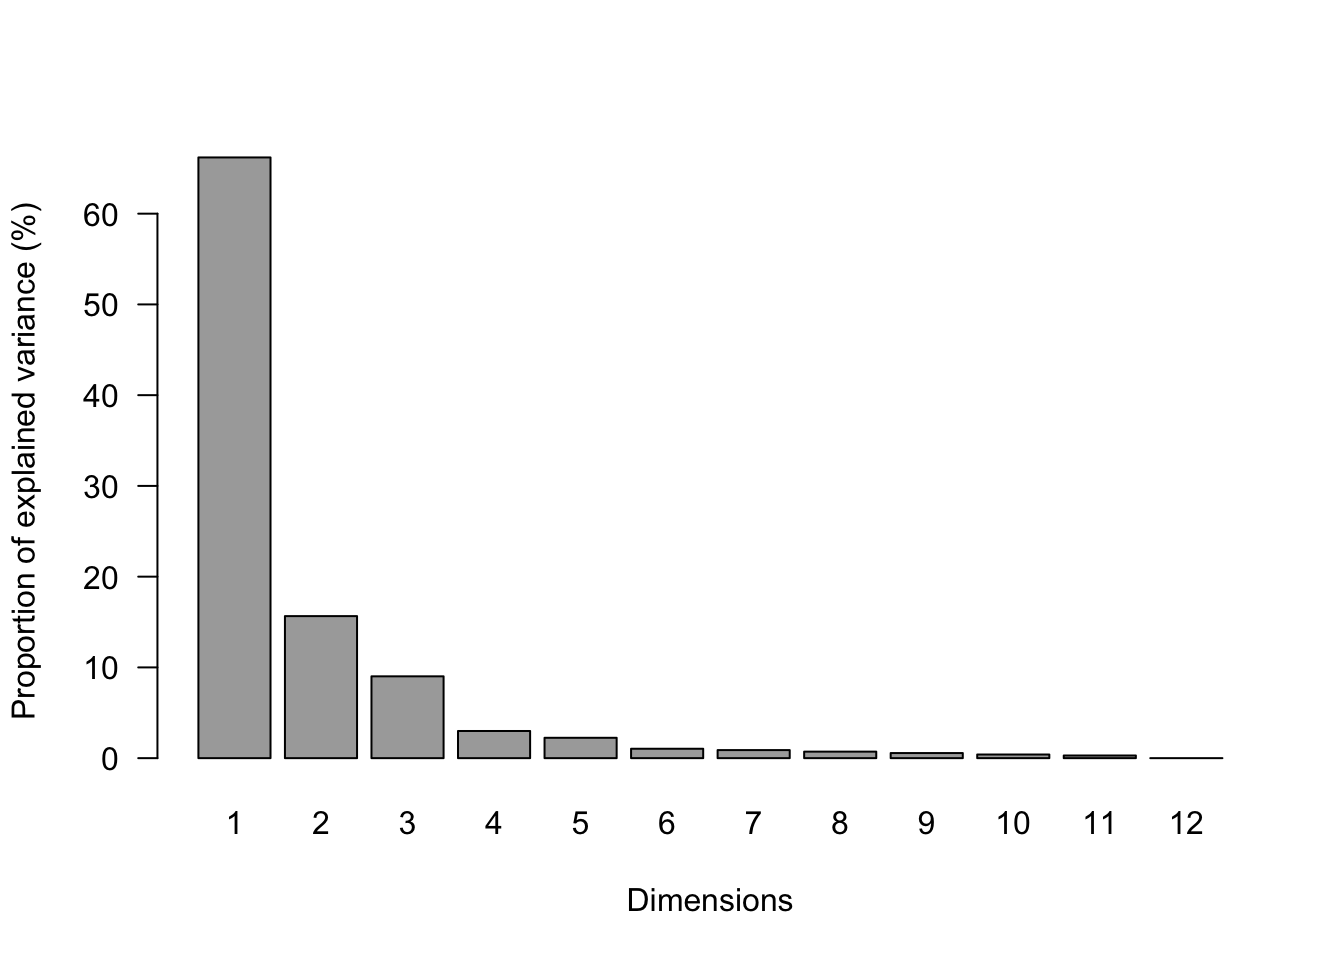
\includegraphics{rna_seq_analysis_files/figure-latex/unnamed-chunk-19-1.pdf}

\begin{Shaded}
\begin{Highlighting}[]
\CommentTok{#all replicates per condition (treatement, location) cluster together!}
\CommentTok{#separation due to treatement, and location!! Need to factor in location!!!}
\end{Highlighting}
\end{Shaded}

\#PCA: Proportion of explained variance transpose the data to have
variables (genes) as columns

\begin{Shaded}
\begin{Highlighting}[]
\NormalTok{data_for_PCA <-}\StringTok{ }\KeywordTok{t}\NormalTok{(dge}\OperatorTok{$}\NormalTok{counts)}
\KeywordTok{dim}\NormalTok{(data_for_PCA)}
\end{Highlighting}
\end{Shaded}

\begin{verbatim}
## [1]    12 21665
\end{verbatim}

\begin{Shaded}
\begin{Highlighting}[]
\CommentTok{## calculate MDS (matrix of dissimilarities)}
\NormalTok{mds <-}\StringTok{ }\KeywordTok{cmdscale}\NormalTok{(}\KeywordTok{dist}\NormalTok{(data_for_PCA), }\DataTypeTok{k=}\DecValTok{3}\NormalTok{, }\DataTypeTok{eig=}\OtherTok{TRUE}\NormalTok{)  }
\CommentTok{# k = the maximum dimension of the space which the data are to be represented in}
\CommentTok{# eig = indicates whether eigenvalues should be returned}
\CommentTok{#mds$eig}

\CommentTok{##How many components can explain the variabilty?}
\CommentTok{# transform the Eigen values into percentage}
\NormalTok{eig_pc <-}\StringTok{ }\NormalTok{mds}\OperatorTok{$}\NormalTok{eig }\OperatorTok{*}\StringTok{ }\DecValTok{100} \OperatorTok{/}\StringTok{ }\KeywordTok{sum}\NormalTok{(mds}\OperatorTok{$}\NormalTok{eig)}
\CommentTok{# plot the PCA}
\CommentTok{#png(file="~/PCA_PropExplainedVariance.png")}
\KeywordTok{barplot}\NormalTok{(eig_pc,}
        \DataTypeTok{las=}\DecValTok{1}\NormalTok{,}
        \DataTypeTok{xlab=}\StringTok{"Dimensions"}\NormalTok{, }
        \DataTypeTok{ylab=}\StringTok{"Proportion of explained variance (%)"}\NormalTok{, }\DataTypeTok{y.axis=}\OtherTok{NULL}\NormalTok{,}
        \DataTypeTok{col=}\StringTok{"darkgrey"}\NormalTok{, }\DataTypeTok{names.arg =} \DecValTok{1}\OperatorTok{:}\DecValTok{12}\NormalTok{)}
\end{Highlighting}
\end{Shaded}

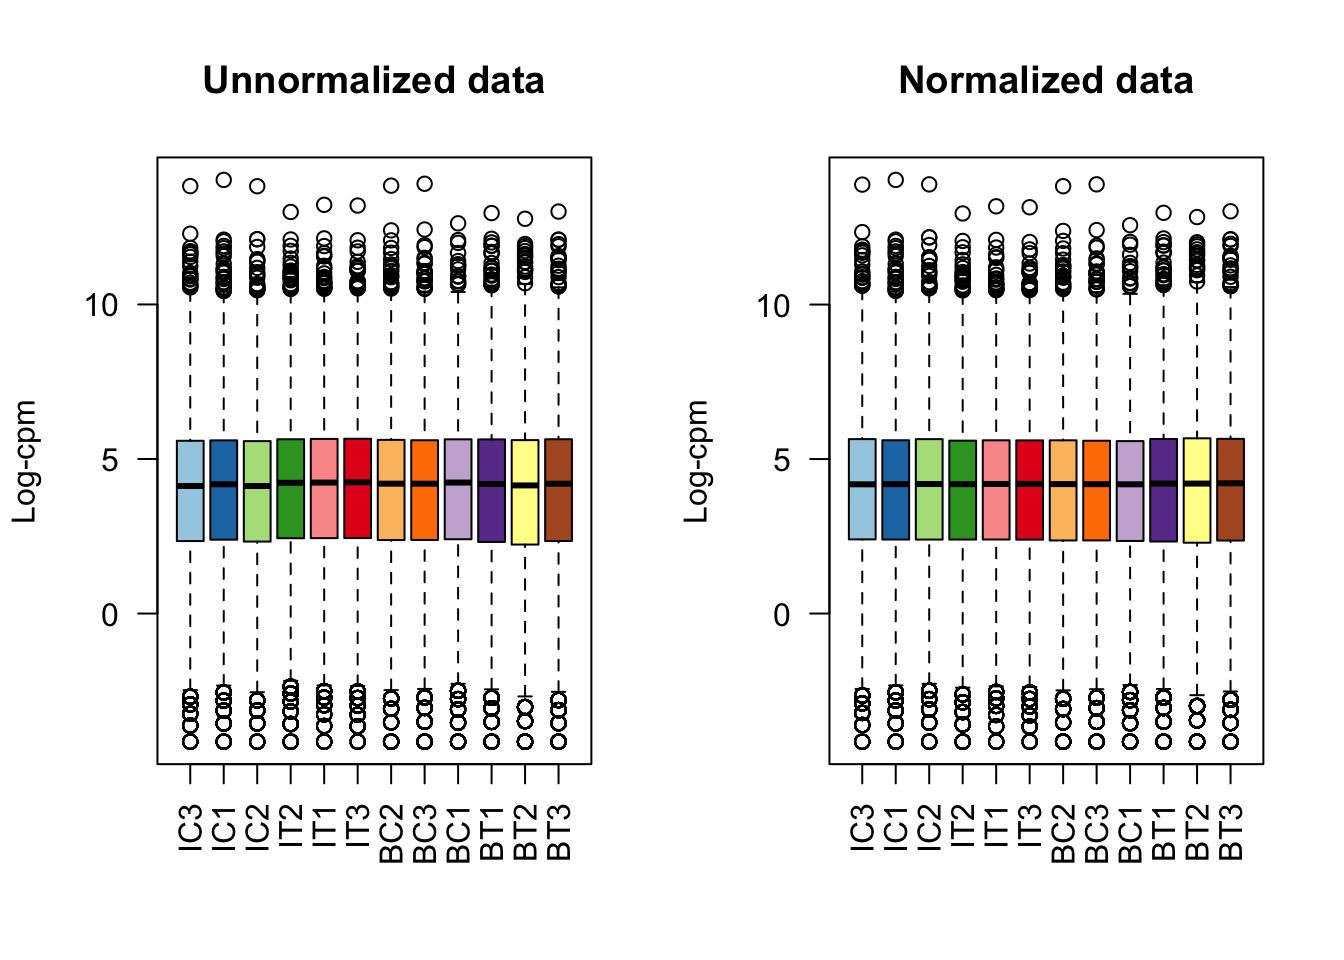
\includegraphics{rna_seq_analysis_files/figure-latex/unnamed-chunk-20-1.pdf}
\#\#LEARNING CHECK: What proportion of variance is explained by
treatment?

\#dev.off()

\#CONCLUSSION: MDS plot support DE analysis between TR and UTR!!!!
\#Suggestive of accounting for location!

\#\#\#STATISTICS!

\#\#FITTING MODELS TO DATA: Fitting genewise negative binomial
generalized linear models (unlike limma lmFit that uses logcpm--assuming
Normality--after adding `voom' weights) create design matrix for
differential expression analysis; if you wanted to account for batch
here, you could simply include a batch term in the linear model at this
step, e.g.: mod \textless- model.matrix(\textasciitilde0 +
fc2\(samples\)lane + fc2\(samples\)group ) \#\#IF WE NEEDED TO ACCOUNT
FOR LANE EFFECTS, IN THIS CASE NO

Create a design matrix fir the linear models \#No reference
group/treatment, and no intercept, easier for pair-wise comparisons with
contrasts (ANOVA-like comparison)

\#METHOD 1: DEGs, for each location, separately: No intercept
(ANOVA-like comparison) Adding intercept-- the first coefficient is the
average value of the control group, the other is the off-set for the
treatment group. No intercept--easier to use contrasts for hypothesis
testing involving multiple comparisons. We will see an example with
intercept in METHOD 2 (location as factor in the model).

\begin{Shaded}
\begin{Highlighting}[]
\NormalTok{mod <-}\StringTok{ }\KeywordTok{model.matrix}\NormalTok{(}\OperatorTok{~}\DecValTok{0}\OperatorTok{+}\NormalTok{dge}\OperatorTok{$}\NormalTok{samples}\OperatorTok{$}\NormalTok{group) }\CommentTok{#no intercept (coefficient for baseline)}
\CommentTok{#mod}
\KeywordTok{rownames}\NormalTok{(mod) <-}\StringTok{ }\KeywordTok{colnames}\NormalTok{(dge)}
\KeywordTok{colnames}\NormalTok{(mod)<-}\KeywordTok{c}\NormalTok{(}\StringTok{"BC"}\NormalTok{,}\StringTok{"BT"}\NormalTok{,}\StringTok{"IC"}\NormalTok{,}\StringTok{"IT"}\NormalTok{)}
\end{Highlighting}
\end{Shaded}

Check the model:

\begin{Shaded}
\begin{Highlighting}[]
\NormalTok{mod}
\end{Highlighting}
\end{Shaded}

\begin{verbatim}
##     BC BT IC IT
## IC3  0  0  1  0
## IC1  0  0  1  0
## IC2  0  0  1  0
## IT2  0  0  0  1
## IT1  0  0  0  1
## IT3  0  0  0  1
## BC2  1  0  0  0
## BC3  1  0  0  0
## BC1  1  0  0  0
## BT1  0  1  0  0
## BT2  0  1  0  0
## BT3  0  1  0  0
## attr(,"assign")
## [1] 1 1 1 1
## attr(,"contrasts")
## attr(,"contrasts")$`dge$samples$group`
## [1] "contr.treatment"
\end{verbatim}

Estimate dispersion:

\begin{Shaded}
\begin{Highlighting}[]
\NormalTok{dge2 <-}\StringTok{ }\KeywordTok{estimateDisp}\NormalTok{(dge, }\DataTypeTok{design =}\NormalTok{ mod )}
\end{Highlighting}
\end{Shaded}

make contrasts: Below, a +ve log FC denotes gene upregulated TR relative
to UTR baseline\\
Recommended if you have many comparisons/contrasts

\begin{Shaded}
\begin{Highlighting}[]
\NormalTok{contr.matrix <-}\StringTok{ }\KeywordTok{makeContrasts}\NormalTok{(}
    \DataTypeTok{Beach_T_vs_Beach_C =}\NormalTok{ BT }\OperatorTok{-}\StringTok{ }\NormalTok{BC,}
    \DataTypeTok{Inland_T_vs_Inland_C =}\NormalTok{ IT }\OperatorTok{-}\StringTok{ }\NormalTok{IC,}
    \DataTypeTok{levels =} \KeywordTok{colnames}\NormalTok{(mod))}
\end{Highlighting}
\end{Shaded}

Check the matrix

\begin{Shaded}
\begin{Highlighting}[]
\NormalTok{contr.matrix}
\end{Highlighting}
\end{Shaded}

\begin{verbatim}
##       Contrasts
## Levels Beach_T_vs_Beach_C Inland_T_vs_Inland_C
##     BC                 -1                    0
##     BT                  1                    0
##     IC                  0                   -1
##     IT                  0                    1
\end{verbatim}

Fit a Generalized Linear Model (GLM):

\begin{Shaded}
\begin{Highlighting}[]
\NormalTok{fit <-}\StringTok{ }\KeywordTok{glmFit}\NormalTok{(dge2, mod)}
\end{Highlighting}
\end{Shaded}

Perform Hypothesis testing (is DE significant?) using Likelihood ratio
test Beach:

\begin{Shaded}
\begin{Highlighting}[]
\NormalTok{  glf_Beach_T_vs_Beach_C <-}\KeywordTok{glmLRT}\NormalTok{(fit, }\DataTypeTok{contrast =}\NormalTok{ contr.matrix[,}\StringTok{"Beach_T_vs_Beach_C"}\NormalTok{])}
\end{Highlighting}
\end{Shaded}

Inland:

\begin{Shaded}
\begin{Highlighting}[]
\NormalTok{  glf_Inland_T_vs_Inland_C <-}\KeywordTok{glmLRT}\NormalTok{(fit, }\DataTypeTok{contrast =}\NormalTok{ contr.matrix[,}\StringTok{"Inland_T_vs_Inland_C"}\NormalTok{])}
\end{Highlighting}
\end{Shaded}

Perform multiple testing correction/p value adjustment. Why? Here:
\url{https://www.ncbi.nlm.nih.gov/pmc/articles/PMC6099145/} First,
interrogate the top DE genes, inland:

\begin{Shaded}
\begin{Highlighting}[]
\KeywordTok{topTags}\NormalTok{(glf_Inland_T_vs_Inland_C)}
\end{Highlighting}
\end{Shaded}

\begin{verbatim}
## Coefficient:  -1*IC 1*IT 
##                      Geneid   Chr    Start      End Strand Length     logFC
## 9569  Phvul.004G056400.v1.0 Chr04  7396606  7397508      -    903  6.196673
## 2632  Phvul.001G263200.v1.0 Chr01 51729773 51729982      +    210  4.512078
## 17196 Phvul.007G231800.v1.0 Chr07 47146783 47148189      -   1407  5.260009
## 15887 Phvul.007G100900.v1.0 Chr07 10966196 10970519      -   4324  2.279606
## 673   Phvul.001G067300.v1.0 Chr01  8642080  8646688      -   4609  4.352858
## 20965 Phvul.009G034300.v1.0 Chr09  7372885  7373614      +    730 -4.680555
## 21686 Phvul.009G106400.v1.0 Chr09 16017975 16023446      +   5472 -2.746245
## 13407 Phvul.006G075000.v1.0 Chr06 19419104 19420608      -   1505  3.977573
## 6999  Phvul.003G096700.v1.0 Chr03 22229474 22230485      -   1012  3.550444
## 754   Phvul.001G075400.v1.0 Chr01 10506529 10509049      -   2521  3.084691
##         logCPM       LR        PValue           FDR
## 9569  4.368390 620.0862 7.161676e-137 1.551577e-132
## 2632  4.083698 483.8931 3.038253e-107 3.291188e-103
## 17196 6.635312 481.2923 1.118259e-106 8.075697e-103
## 15887 5.402644 387.8966  2.375728e-86  1.286754e-82
## 673   6.778686 386.2670  5.377384e-86  2.330020e-82
## 20965 4.016624 372.2606  6.025646e-83  2.175760e-79
## 21686 6.529474 346.8216  2.085873e-77  6.455777e-74
## 13407 6.495196 324.1158  1.838235e-72  4.978169e-69
## 6999  3.873551 318.1419  3.678151e-71  8.854128e-68
## 754   6.171969 317.7187  4.548098e-71  9.853454e-68
\end{verbatim}

Get all DE genes with adjusted p.value cutoff (Inland)

\begin{Shaded}
\begin{Highlighting}[]
\NormalTok{pvals_T_vs_C_inland<-}\KeywordTok{topTags}\NormalTok{(glf_Inland_T_vs_Inland_C, }\DataTypeTok{n =} \StringTok{"Inf"}\NormalTok{, }\DataTypeTok{adjust.method =} \StringTok{"BH"}\NormalTok{, }\DataTypeTok{sort.by =} \StringTok{"PValue"}\NormalTok{, }\DataTypeTok{p.value =} \FloatTok{0.1}\NormalTok{ )}
\NormalTok{pvals_T_vs_C_inland<-pvals_T_vs_C_inland[[}\DecValTok{1}\NormalTok{]] }\CommentTok{#get the dataframe, from the edgeR object}
\end{Highlighting}
\end{Shaded}

Count genes with FDF\textless=0.1, but consider different FDRs use the
data wrangling package `dplyr', included in `tidyverse' package see top
10 genes, with FDR cutoff of 0.1

\begin{Shaded}
\begin{Highlighting}[]
\NormalTok{pvals_T_vs_C_inland }\OperatorTok
\StringTok{  }\NormalTok{dplyr}\OperatorTok{::}\KeywordTok{filter}\NormalTok{(FDR }\OperatorTok{<=}\StringTok{ }\FloatTok{0.1}\NormalTok{) }\OperatorTok
\StringTok{  }\KeywordTok{head}\NormalTok{(}\DecValTok{10}\NormalTok{)}
\end{Highlighting}
\end{Shaded}

\begin{verbatim}
##                      Geneid   Chr    Start      End Strand Length     logFC
## 9569  Phvul.004G056400.v1.0 Chr04  7396606  7397508      -    903  6.196673
## 2632  Phvul.001G263200.v1.0 Chr01 51729773 51729982      +    210  4.512078
## 17196 Phvul.007G231800.v1.0 Chr07 47146783 47148189      -   1407  5.260009
## 15887 Phvul.007G100900.v1.0 Chr07 10966196 10970519      -   4324  2.279606
## 673   Phvul.001G067300.v1.0 Chr01  8642080  8646688      -   4609  4.352858
## 20965 Phvul.009G034300.v1.0 Chr09  7372885  7373614      +    730 -4.680555
## 21686 Phvul.009G106400.v1.0 Chr09 16017975 16023446      +   5472 -2.746245
## 13407 Phvul.006G075000.v1.0 Chr06 19419104 19420608      -   1505  3.977573
## 6999  Phvul.003G096700.v1.0 Chr03 22229474 22230485      -   1012  3.550444
## 754   Phvul.001G075400.v1.0 Chr01 10506529 10509049      -   2521  3.084691
##         logCPM       LR        PValue           FDR
## 9569  4.368390 620.0862 7.161676e-137 1.551577e-132
## 2632  4.083698 483.8931 3.038253e-107 3.291188e-103
## 17196 6.635312 481.2923 1.118259e-106 8.075697e-103
## 15887 5.402644 387.8966  2.375728e-86  1.286754e-82
## 673   6.778686 386.2670  5.377384e-86  2.330020e-82
## 20965 4.016624 372.2606  6.025646e-83  2.175760e-79
## 21686 6.529474 346.8216  2.085873e-77  6.455777e-74
## 13407 6.495196 324.1158  1.838235e-72  4.978169e-69
## 6999  3.873551 318.1419  3.678151e-71  8.854128e-68
## 754   6.171969 317.7187  4.548098e-71  9.853454e-68
\end{verbatim}

bottom DE genes:

\begin{Shaded}
\begin{Highlighting}[]
\NormalTok{pvals_T_vs_C_inland }\OperatorTok
\StringTok{  }\NormalTok{dplyr}\OperatorTok{::}\KeywordTok{filter}\NormalTok{(FDR }\OperatorTok{<=}\StringTok{ }\FloatTok{0.1}\NormalTok{) }\OperatorTok
\StringTok{  }\KeywordTok{tail}\NormalTok{()}
\end{Highlighting}
\end{Shaded}

\begin{verbatim}
##                      Geneid   Chr    Start      End Strand Length      logFC
## 16452 Phvul.007G157400.v1.0 Chr07 38261335 38265910      -   4576  0.1688971
## 24722 Phvul.010G146700.v1.0 Chr10 41800513 41805539      +   5027  0.2880521
## 4416  Phvul.002G172200.v1.0 Chr02 31918896 31924015      +   5120 -0.4263375
## 21812 Phvul.009G119000.v1.0 Chr09 17679640 17684688      -   5049 -0.1949631
## 7289  Phvul.003G125700.v1.0 Chr03 30689612 30692651      -   3040 -0.3560639
## 17073 Phvul.007G219500.v1.0 Chr07 45905776 45906185      +    410 -0.3494290
##         logCPM       LR     PValue        FDR
## 16452 7.040785 4.375717 0.03645448 0.09978350
## 24722 4.488565 4.374547 0.03647952 0.09983943
## 4416  2.735681 4.373171 0.03650899 0.09990746
## 21812 4.743594 4.372324 0.03652715 0.09994451
## 7289  5.623442 4.371984 0.03653444 0.09995184
## 17073 5.200892 4.371143 0.03655247 0.09998856
\end{verbatim}

get the number of genes with FDR cutoff of 0.1

\begin{Shaded}
\begin{Highlighting}[]
\NormalTok{pvals_T_vs_C_inland }\OperatorTok
\StringTok{  }\KeywordTok{filter}\NormalTok{(FDR }\OperatorTok{<=}\StringTok{ }\FloatTok{0.1}\NormalTok{) }\OperatorTok
\StringTok{  }\KeywordTok{count}\NormalTok{() }
\end{Highlighting}
\end{Shaded}

\begin{verbatim}
##      n
## 1 7920
\end{verbatim}

\#Useful graphical representations of differential expression results
Get number of up and down regulated genes:

\begin{Shaded}
\begin{Highlighting}[]
\NormalTok{dt<-}\KeywordTok{decideTests}\NormalTok{(glf_Inland_T_vs_Inland_C, }\DataTypeTok{adjust.method =} \StringTok{"BH"}\NormalTok{, }\DataTypeTok{p.value =} \FloatTok{0.1}\NormalTok{)}
\KeywordTok{summary}\NormalTok{(dt)}
\end{Highlighting}
\end{Shaded}

\begin{verbatim}
##        -1*IC 1*IT
## Down         4006
## NotSig      13745
## Up           3914
\end{verbatim}

\#Get gene IDs (ENSEMBLE) of DE genes de.genes \textless-
which(dt{[},1{]}!=0) \#DE genes, 0 represents not DE genes de.genes
length(de.genes)

Mean-difference plot. Significantly DE genes at a FDR of 5\% are
highlighted

with ggplot

\begin{Shaded}
\begin{Highlighting}[]
\KeywordTok{library}\NormalTok{(ggplot2)}
\CommentTok{#create a dataframe with 'sign' column showing Up, Down, or Non.sig}
\NormalTok{sign.dat<-glf_Inland_T_vs_Inland_C}\OperatorTok{$}\NormalTok{table }\OperatorTok
\StringTok{  }\NormalTok{dplyr}\OperatorTok{::}\KeywordTok{mutate}\NormalTok{(}\DataTypeTok{sign=}\KeywordTok{case_when}\NormalTok{(logFC}\OperatorTok{>}\DecValTok{0} \OperatorTok{&}\StringTok{ }\NormalTok{PValue }\OperatorTok{<}\StringTok{ }\FloatTok{0.05} \OperatorTok{~}\StringTok{ "Up"}\NormalTok{,}
\NormalTok{                               logFC}\OperatorTok{<}\DecValTok{0} \OperatorTok{&}\StringTok{ }\NormalTok{PValue }\OperatorTok{<}\StringTok{ }\FloatTok{0.05} \OperatorTok{~}\StringTok{ "Down"}\NormalTok{,}
\NormalTok{                               PValue }\OperatorTok{>}\StringTok{ }\FloatTok{0.05} \OperatorTok{~}\StringTok{ "Non.sigf"}\NormalTok{)}
\NormalTok{                )}

\CommentTok{#head(sign.dat)}
\KeywordTok{ggplot}\NormalTok{(sign.dat, }\KeywordTok{aes}\NormalTok{(}\DataTypeTok{x =}\NormalTok{ logCPM, }\DataTypeTok{y=}\NormalTok{logFC,}\DataTypeTok{col=}\NormalTok{sign)) }\OperatorTok{+}
\CommentTok{#  geom_point(alpha=0.4) + }
\StringTok{  }\KeywordTok{geom_point}\NormalTok{() }\OperatorTok{+}\StringTok{ }
\StringTok{  }\KeywordTok{scale_colour_manual}\NormalTok{(}\DataTypeTok{values=}\KeywordTok{c}\NormalTok{(}\StringTok{"blue"}\NormalTok{,}\StringTok{"black"}\NormalTok{,}\StringTok{"red"}\NormalTok{)) }\OperatorTok{+}\StringTok{ }
\StringTok{  }\KeywordTok{labs}\NormalTok{(}\DataTypeTok{x =} \StringTok{"Average log CPM"}\NormalTok{, }\DataTypeTok{y =} \StringTok{"log-fold-change"}\NormalTok{) }\OperatorTok{+}
\StringTok{  }\KeywordTok{theme}\NormalTok{(}\DataTypeTok{legend.position =} \KeywordTok{c}\NormalTok{(}\FloatTok{0.9}\NormalTok{, }\FloatTok{0.9}\NormalTok{), }\DataTypeTok{legend.title =} \KeywordTok{element_blank}\NormalTok{()) }\OperatorTok{+}
\StringTok{  }\KeywordTok{theme}\NormalTok{(}
    \DataTypeTok{axis.title.x =} \KeywordTok{element_text}\NormalTok{(}\DataTypeTok{size=}\DecValTok{14}\NormalTok{),}
    \DataTypeTok{axis.title.y =} \KeywordTok{element_text}\NormalTok{(}\DataTypeTok{size=}\DecValTok{14}\NormalTok{), }
    \DataTypeTok{axis.text.x =} \KeywordTok{element_text}\NormalTok{(}\DataTypeTok{size =} \DecValTok{14}\NormalTok{), }
    \DataTypeTok{axis.text.y =} \KeywordTok{element_text}\NormalTok{(}\DataTypeTok{size =} \DecValTok{14}\NormalTok{)}
\NormalTok{  )}
\end{Highlighting}
\end{Shaded}

\includegraphics{rna_seq_analysis_files/figure-latex/unnamed-chunk-35-1.pdf}

Interactive MD plot

\begin{Shaded}
\begin{Highlighting}[]
\CommentTok{#install Glimma package}
\CommentTok{#if (!requireNamespace("BiocManager", quietly = TRUE))}
\CommentTok{#  install.packages("BiocManager")}
\CommentTok{#BiocManager::install("Glimma")}

\KeywordTok{library}\NormalTok{(Glimma)}
\KeywordTok{glMDPlot}\NormalTok{(glf_Inland_T_vs_Inland_C, }\DataTypeTok{coef=}\DecValTok{1}\NormalTok{, }\DataTypeTok{status=}\NormalTok{dt, }\DataTypeTok{main=}\KeywordTok{colnames}\NormalTok{(glf_Inland_T_vs_Inland_C)[}\DecValTok{1}\NormalTok{],}
         \DataTypeTok{side.main=}\StringTok{"ENTREZID"}\NormalTok{, }\DataTypeTok{counts=}\NormalTok{lcpm, }\DataTypeTok{groups=}\NormalTok{glf_Inland_T_vs_Inland_C}\OperatorTok{$}\NormalTok{samples}\OperatorTok{$}\NormalTok{group, }\DataTypeTok{launch=}\OtherTok{TRUE}\NormalTok{)}
\end{Highlighting}
\end{Shaded}

Heatmap of the top 100 DE genes

\begin{Shaded}
\begin{Highlighting}[]
\CommentTok{#install.packages("gplots")}
\KeywordTok{library}\NormalTok{(gplots)}
\end{Highlighting}
\end{Shaded}

\begin{verbatim}
## 
## Attaching package: 'gplots'
\end{verbatim}

\begin{verbatim}
## The following object is masked from 'package:stats':
## 
##     lowess
\end{verbatim}

\begin{Shaded}
\begin{Highlighting}[]
\NormalTok{tr.vs.utr.topgenes <-}\StringTok{ }\NormalTok{pvals_T_vs_C_inland}\OperatorTok{$}\NormalTok{Geneid[}\DecValTok{1}\OperatorTok{:}\DecValTok{100}\NormalTok{] }\CommentTok{#get IDS of top DEGs}
\NormalTok{i <-}\StringTok{ }\KeywordTok{which}\NormalTok{(dge}\OperatorTok{$}\NormalTok{genes}\OperatorTok{$}\NormalTok{Geneid }\OperatorTok\StringTok{ }\NormalTok{tr.vs.utr.topgenes) }\CommentTok{#Get their index in the expression table}
\NormalTok{mycol <-}\StringTok{ }\KeywordTok{colorpanel}\NormalTok{(}\DecValTok{1000}\NormalTok{,}\StringTok{"blue"}\NormalTok{,}\StringTok{"white"}\NormalTok{,}\StringTok{"red"}\NormalTok{)}
\KeywordTok{heatmap.2}\NormalTok{(lcpm[i,], }\DataTypeTok{scale=}\StringTok{"row"}\NormalTok{,}
          \DataTypeTok{labRow=}\NormalTok{dge}\OperatorTok{$}\NormalTok{genes}\OperatorTok{$}\NormalTok{Geneid[i], }\DataTypeTok{labCol=}\NormalTok{dge}\OperatorTok{$}\NormalTok{samples}\OperatorTok{$}\NormalTok{group,}
          \DataTypeTok{col=}\NormalTok{mycol, }\DataTypeTok{trace=}\StringTok{"none"}\NormalTok{, }\DataTypeTok{density.info=}\StringTok{"none"}\NormalTok{, }\DataTypeTok{dendrogram=}\StringTok{"column"}\NormalTok{)}
\end{Highlighting}
\end{Shaded}

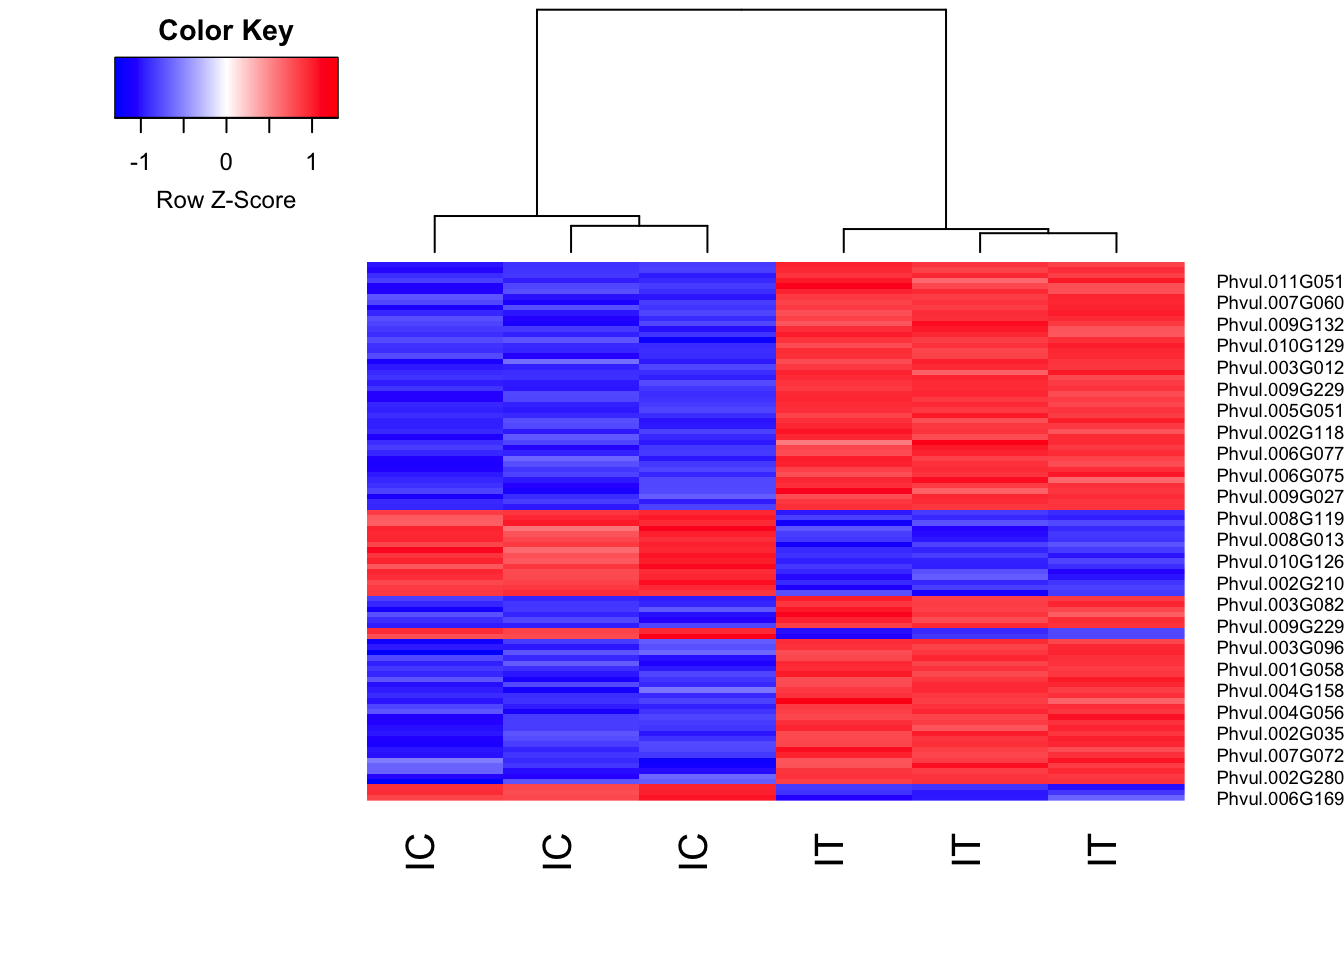
\includegraphics{rna_seq_analysis_files/figure-latex/unnamed-chunk-37-1.pdf}

The above heatmap has samples from all locations, our interest for now
is inland. However, looks like (as expected), all treatment samples are
clustering together, irrespective of location.

LEARNING CHECK: Produce a heatmap with inland samples only (hint: index
only relevant samples in the expression matrix for plotting) SOLUTION
(HIDE)

\begin{Shaded}
\begin{Highlighting}[]
\CommentTok{#install.packages("gplots")}
\NormalTok{tr.vs.utr.topgenes <-}\StringTok{ }\NormalTok{pvals_T_vs_C_inland}\OperatorTok{$}\NormalTok{Geneid[}\DecValTok{1}\OperatorTok{:}\DecValTok{100}\NormalTok{] }\CommentTok{#get IDS of top DEGs}
\NormalTok{i <-}\StringTok{ }\KeywordTok{which}\NormalTok{(dge}\OperatorTok{$}\NormalTok{genes}\OperatorTok{$}\NormalTok{Geneid }\OperatorTok\StringTok{ }\NormalTok{tr.vs.utr.topgenes) }\CommentTok{#Get their index in the expression table}
\NormalTok{mycol <-}\StringTok{ }\KeywordTok{colorpanel}\NormalTok{(}\DecValTok{1000}\NormalTok{,}\StringTok{"blue"}\NormalTok{,}\StringTok{"white"}\NormalTok{,}\StringTok{"red"}\NormalTok{)}
\KeywordTok{heatmap.2}\NormalTok{(lcpm[i,}\DecValTok{1}\OperatorTok{:}\DecValTok{6}\NormalTok{], }\DataTypeTok{scale=}\StringTok{"row"}\NormalTok{,}
          \DataTypeTok{labRow=}\NormalTok{dge}\OperatorTok{$}\NormalTok{genes}\OperatorTok{$}\NormalTok{Geneid[i], }\DataTypeTok{labCol=}\NormalTok{dge}\OperatorTok{$}\NormalTok{samples}\OperatorTok{$}\NormalTok{group,}
          \DataTypeTok{col=}\NormalTok{mycol, }\DataTypeTok{trace=}\StringTok{"none"}\NormalTok{, }\DataTypeTok{density.info=}\StringTok{"none"}\NormalTok{, }\DataTypeTok{dendrogram=}\StringTok{"column"}\NormalTok{)}
\end{Highlighting}
\end{Shaded}

\includegraphics{rna_seq_analysis_files/figure-latex/unnamed-chunk-38-1.pdf}

\#LEARNING CHECK: 1. What is the number of DEGs on the beach? 2. How
many of the beach DEGs are also DEGs inland?

\end{document}
